%===========================================================
%                              Choix de track
%===========================================================
% Une des trois options 'parallelisme', 'architecture', 'systeme' 
% doit être utilisée avec le style compas2016
\documentclass[parallelisme]{compas2016}

\usepackage[utf8]{inputenc}
\usepackage[T1]{fontenc}

\usepackage{url}
\usepackage{graphicx}
\usepackage{caption}
\usepackage{subcaption}
\usepackage{subfig}
\usepackage{wrapfig}
\usepackage{multirow}
\usepackage{boxedminipage}
\usepackage{xspace}
\usepackage{listings}
\usepackage{listingsutf8}
\usepackage{verbatim}
\usepackage{parcolumns}
\usepackage{color}
\usepackage[usenames,dvipsnames,svgnames,table]{xcolor}
%Prevents floating item to "jump" between sections
\usepackage[section]{placeins}
\usepackage{booktabs}
\usepackage{tkz-graph}
\usepackage{setspace}
%\setstretch{0.95}




\renewcommand{\ttdefault}{pcr}
\lstset{
	tabsize=4,
%	frame=single,
	breaklines=true,
	basicstyle=\ttfamily,
	frame=tb,
	framerule=0.2pt,
%	frameround={tttt},
	showstringspaces=false,
	language=c,
%	linewidth=0.95\textwidth,
	keywordstyle=\color{black}\bfseries,
%	keywordstyle=\color{blue},
	commentstyle=\color{OliveGreen},
	stringstyle=\color{red}\itshape,
	inputencoding=utf8/latin1,
	numbers=left,
	numberstyle=\tiny,
	numbersep=5pt,
% OMP define
emph={\#,pragma, taskwait, omp, task, depend}, emphstyle=\color{RoyalBlue}\bfseries,
emph={[2]in,inout,out,cw}, emphstyle={[2]\color{BrickRed}\bfseries},
emph={[3]tied,untied,shared}, emphstyle={[3]\color{Gray}\bfseries},
emph={[4]lu0,fwd,bdiv,bmod}, emphstyle={[4]\color{DarkGreen}\bfseries},
emph={[5]cw}, emphstyle={[5]\color{DarkViolet}\bfseries},
    %moredelim=**[is][\only<3>{\color{red}}]{@}{@},
}
\lstdefinestyle{smaller}{basicstyle=\scriptsize\ttfamily}
\lstMakeShortInline|
%===========================================================
%                               Title
%===========================================================

\toappear{1} % Conserver cette ligne pour la version finale

\begin{document}

\title{Amélioration des stratégies d'ordonnancement sur architectures NUMA à l'aide
des dépendances de données}

\author{Philippe Virouleau}
\address{Inria,\\
   Univ. Grenoble Alpes,  CNRS, Grenoble Institute of Technology, LIG, Grenoble, France\\
   philippe.virouleau@inria.fr\\
}
\date{}


\maketitle

\newcommand{\benchs}{KASTORS }
\newcommand{\kaapi}{\textsc{\mbox{Xkaapi}}\xspace}
%===========================================================         %
%R\'esum\'e
%===========================================================  
\begin{abstract}
Le récent ajout des dépendances de données à la norme OpenMP 4.0 offre
au programmeur une manière flexible de synchroniser les tâches.
Grâce à cela, le compilateur et le support exécutif peuvent tous les deux savoir
exactement quelles données sont lues ou écrites par quelles tâches, et comment
ces données peuvent éventuellement être réutilisées au cours de l'exécution du
programme.
Les performances sur architectures NUMA peuvent être fortement impactées par
le placement des données et l'ordonnancement des tâches. Les informations présentes
dans les dépendances de données peuvent être utilisées pour contrôler le placement physique des données,
ainsi que pour contrôler les stratégies de placement des tâches en
fonction de la topologie.
Ce papier présente plusieurs heuristiques pour ces stratégies, et leurs implémentations
dans notre support exécutif OpenMP : \kaapi.
Nous présentons également nos évaluations sur des applications d'algèbre linéaire,
exécutées sur une machine NUMA à 192 cœurs, et comparées aux stratégies proposées
par l'état de l'art.
  \MotsCles{OpenMP, tâche avec dépendances, support exécutif, NUMA, ordonnancement}
\end{abstract}

	
\section{Introduction}

Bien que les architectures à temps d'accès mémoire non uniforme (NUMA) soient
aujourd'hui l'un des choix les plus populaire pour créer des grosses machines à mémoire
partagées, il est toujours compliqué de pouvoir les exploiter à leur plein potentiel.
Compte tenu de la différence de temps d'accès en fonction de la distribution physique
de la mémoire (une donnée proche sera accédée beaucoup plus rapidement qu'une donnée distante),
contrôler le placement des données tout au long de l'exécution d'une application
est donc l'un des points clés pour améliorer sa scalabilité et ses performances.

Les environnements de programmation parallèle tels que OpenMP sont devenus très
populaires pour exploiter les machines à mémoire partagée avec plusieurs centaines de cœurs.
Ils offrent un moyen d'exprimer beaucoup de parallélisme à grain fin, tout en
ayant un coût relativement faible. La plupart d'entre eux fournissent également
un moyen d'équilibrer dynamiquement la charge de travail sur tous les processeurs,
mais les plus standard ne fournissent pas de moyen explicite de gérer la localité
des données sur des systèmes NUMA.

L'ajout récent des dépendances de données au modèle de programmation par tâches
d'OpenMP fourni au support exécutif des informations précises, notamment concernant
quelle partie de l'application utilise quelle donnée.
L'ordonnanceur de tâches peut donc se baser sur ces informations pour affecter
les tâches aux processeurs, et implémenter des stratégies dédiées aux architectures
NUMA, comme montré dans ce papier.

Ce papier décrit plusieurs stratégies que nous avons implémenté dans notre support
exécutif \kaapi. Nous avons identifié trois points majeurs dans l'ordonnanceur qui
peuvent impacter les applications parallèles pour systèmes NUMA : la distribution
de données, l'assignation des tâches prête, et la manière de parcourir l'architecture
pour effectuer l'équilibrage de charge.

Ce papier les décrit et les évalue, en montrant leur impact sur les performances
d'applications s'exécutant sur une machine NUMA à 192 cœurs.
Nous les comparons également aux stratégies de l'état de l'art implémentées dans \kaapi.

Le plan de ce papier est le suivant : dans la partie~\ref{sec:background},
nous donnons quelques informations essentielles sur les architectures NUMA et
le modèle de tâches avec dépendances. Ensuite dans la partie~\ref{sec:contributions}
nous décrivons les idées, stratégies, et détails d'implémentation que nous avons
utilisé pour améliorer les performances du système exécutif. La partie~\ref{sec:performances-evaluation}
présente les évaluations de performances. Enfin nous présentons des travaux de l'état
de l'art dans la partie~\ref{sec:related-work}, avant de conclure.


\section{Description des systèmes NUMA et de leur exploitation}

\label{sec:background}
\subsection{La couche matérielle}
\label{sec:hardware}
La plupart des architectures à mémoire partagée actuelles sont basées sur le modèle NUMA,
dans lequel la mémoire est physiquement répartie sur plusieurs nœuds attachés
aux processeurs. La plupart des vendeurs relient ces nœuds suivant une logique
hiérarchique, ce qui permet de construire des machines à plusieurs centaines de cœurs.

Le temps d'accès à de la mémoire située sur un nœud local est plus rapide que celui
pour accéder à de la mémoire située sur un nœud distant, il est donc important
de le prendre en compte lors de l'exécution du programme.

Nous avons effectué nos expériences sur une machine SGI UV2000, constituée de
24 nœuds NUMA, possédant chacun un processeur Intel Xeon E5-4640 à 8 cœurs,
le tout formant un total de 192 cœurs. Nous utilisons le nom Intel192 pour faire
référence à cette machine dans le papier.

\subsection{La couche logicielle}

Afin d'exploiter les grosses architectures à mémoire partagée, le programmeur a besoin :
\begin{enumerate}
    \item d'exprimer beaucoup de parallélisme à grain fin, pour profiter au maximum du nombre
      important de processeurs disponibles;
    \item de contrôler l'exécution de l'application, en particulier la manière dont sont distribuées
      les données.
\end{enumerate}

Les environnements de programmation parallèle à base de tâches fournissent un moyen
d'exprimer le parallélisme à grain fin. OpenMP~\cite{openmp40}, le standard utilisé
en pratique pour la programmation des architectures à mémoire partagée, supporte
le parallélisme à base de tâches avec dépendances de données depuis la version 4.0.

\subsubsection{Un aperçu du modèle de tâches d'OpenMP}

Une \emph{tâche} OpenMP peut être vue comme une \emph{unité indépendante de travail} qu'un thread
OpenMP peut exécuter. Les tâches peuvent être exécutées par un thread quelconque
de la région parallèle.
Gérer les tâches pendant l'exécution est bien moins coûteux que de créer et synchroniser
des threads, le programmeur peut donc considérer que certaines parties de son code
trop petites pour être parallélisées avec des threads peuvent l'être avec des tâches.

Dans la norme OpenMP 3.0, la synchronisation des tâches est effectuée à l'aide du
mot clé |taskwait|, imposant l'attente de la complétion de toutes les tâches
de la région parallèle courante.

La norme 4.0 enrichie ce concept en introduisant le mot clé |depend|, qui permet
de spécifier le mode d'accès des variables utilisées par une tâches pendant son exécution.
Le mode d'accès peut être soit |in|, |out|, ou |inout|, en fonction de si la
variable correspondante est respectivement lue par la tâche, écrite, ou bien les deux.
Cette information peut être analysée par le support exécutif, qui décidera si
la tâche est prête à être exécutée ou si elle doit attendre la complétion d'une
autre tâche.


%\subsubsection{Un exemple de la suite de benchmarks KASTORS}
%La figure~\ref{lulst} montre l'implémentation d'une factorisation de Cholesky
%à l'aide des tâches avec dépendances d'OpenMP.
%Cet algorithme est très proche de celui implémenté dans la suite de benchmark
%KASTORS~\cite{virouleau:hal-01081974}, utilisée dans nos expérimentations.

%Dans certaines situations, la programmation par tâches avec dépendances permet
%plusieurs scénarios d'exécution valide de l'application, ce qui permet au
%support exécutif plus de liberté dans l'ordonnancement des tâches.
%Dans l'exemple, il y a plusieurs instances des BLAS |dtrsm|, |dsyrk|, et |dgemm|
%qui peuvent s'exécuter de manière concurrente.

%\begin{figure}[tbp]
%\hrule
%\begin{minipage}[t]{.43\textwidth}
%\begin{lstlisting}[frame=none,style=smaller,showlines=true,label=lst:LU-deps]{lst:LU-deps1}
%for (size_t k=0; k < NB; ++k) {
%#pragma omp task shared(A) \
  %depend(inout: A[k][k])
  %dpotrf(NB,&A[k][k]);

  %for (int m=k; m < NB; ++m) 
%#pragma omp task shared(A)\
  %depend(in: A[k][k]) \
  %depend(inout: A[m][k])
    %dtrsm(NB,&A[k][k],&A[m][k]);

%\end{lstlisting}
%\end{minipage}\hfill
%\begin{minipage}[t]{.485\textwidth}
%\begin{lstlisting}[frame=none,style=smaller,label=lst:LU-deps,firstnumber=12]{lst:LU-deps2}
  %for (int m=k; m < NB; ++m) {
%#pragma omp task shared(A)\
  %depend(in: A[m][k]) \
  %depend(inout: A[m][m])
   %dsyrk(NB,&A[m][k], &A[m][m]);

    %for (int n=k; n < m; ++n)
%#pragma omp task shared(A)\
  %depend(in: A[m][k],A[n][k])\
  %depend(inout: A[m][n])
     %dgemm(NB,
       %&A[m][k],&A[n][k],&A[m][n]);
  %}
 %}
%\end{lstlisting}
%\end{minipage}
%\hrule
%\caption{Cholesky factorization with OpenMP-4.0 task dependencies} \label{lulst}
%\end{figure}


\subsubsection{Notre manière d'exécuter les programmes à base de tâches}

Le support exécutif que nous développons, \kaapi, implémente un modèle d'exécution par vol
de travail pour les programmes à base de tâches OpenMP. Ce modèle a été présenté
à la base dans Cilk~\cite{cilk5}, et est couramment utilisé dans les environnements
de programmation à base de tâches.

\kaapi créer un thread, appelé un \emph{kproc}, pour chaque unité d'exécution
(dans le cas d'une machine NUMA, il s'agit d'un cœur).
Chaque kproc possède sa propre queue de travail dans laquelle il poussera les
tâches qu'il créer, et qui est implémentée comme une pile,

Le graphe de dépendances est construit, et lors d'un vol le voleur va choisir
l'une des tâches dans la liste des tâches prêtes de la victime.
C'est lors de ce vol qu'on va notamment pouvoir mettre en place des stratégies
adaptées aux architectures NUMA.




\section{Amélioration du placement des tâches et des données grâce aux dépendances}
\label{sec:contributions}

Dans cette partie, nous décrivons comment le support exécutif peut avoir un impact
positif sur l'exécution de l'application, en utilisant les informations présentes
dans les dépendances.


\vspace*{-1ex}
\subsection{La mécanique interne de \kaapi}

Les paragraphes suivant décrivent quelques mécanismes clés du support exécutif \kaapi.


\vspace*{-1ex}
\subsubsection{Modélisation de l'architecture}

\kaapi modélise la topologie de l'architecture comme une hiérarchie de \verb/places/.
Une \verb/place/ est en fait une liste de tâches associées à un ensemble de cœurs.
La plupart du temps \kaapi considère deux niveaux de places : les places de niveau
NUMA (une place par nœud NUMA, regroupant l'ensemble des cœurs sur ce nœud),
et les places au niveau du processeur (une place par cœur).


\subsubsection{La manière de voler des tâches prêtes}

L'environnement de développement dans \kaapi~\cite{Bleuse2014} repose sur des fonctions
virtuelles pour \textit{sélectionner une victime}, \textit{sélectionner une place} dans
laquelle pousser une tâche prête, et \textit{pousser} un ensemble de tâches initialement
prêtes.
Quand un processeur devient inactif, le support exécutif utilise une fonction appelée
\verb/WSselect/ pour parcourir la topologie à la recherche d'une place à voler.

La complétion d'une tâche peut rendre possible l'exécution d'un ensemble de tâches.
Le choix de la place où pousser chacune des tâches est implémentée par une fonction
appelée \verb/WSpush/.
Avant l'exécution parallèle de l'application, le support exécutif peut répartir
les tâches prêtes à l'aide de la fonction appelée \verb/WSpush_init/.

Ces trois fonctions sont les trois points d'entrée à préciser pour définir
un algorithme d'ordonnancement dans \kaapi.


\subsection{Contrôler la distribution de donnée sur les architectures NUMA}

Contrôler le placement des données nécessite de bien connaître l'architecture NUMA.
Les programmeurs peuvent contrôler l'allocation des données à l'aide d'outils
dédiés, tels que \verb/numactl/~\cite{DBLP:journals/corr/abs-1101-0093}.

Par exemple l'option \verb/--interleave=all/ permet de répartir toutes les pages
sur l'architecture suivant une politique de round-robin sur tous les nœuds NUMA.
Cette politique est largement utilisé avec du parallélisme dynamique sur systèmes
NUMA, car elle répartie le trafic mémoire sur tous les contrôleurs mémoire, rendant
tous les processeurs "\emph{équitablement mauvais}" par rapport aux accès mémoire.

Nous proposons deux approches différentes pour distribuer la mémoire sur les systèmes
NUMA, basé sur le principe de l'allocation \emph{first-touch} de la mémoire :
\begin{itemize}
  \item Soit le programmeur peut allouer explicitement la donnée sur un nœud NUMA
    spécifique de la machine, via une API que nous fournissons~\cite{Durand2013}.
    Cela peut être par exemple une distribution cyclique par bloc, ou par bloc à
    deux dimensions comme MAMI~\cite{BroFurGogWacNam10IJPP}.
  \item ou alors le programmeur peut marquer certaines portions de code comme
    étant du code d'initialisation, et le support exécutif se charge de la distribution
    des tâches créées dans cette portion.
    Olivier et al.~\cite{Olivier:2012:CMW:2388996.2389085} ont utilisés cette
    approche avec des restrictions sur l'exécution des tâches créées par l'application.
\end{itemize}

Ces deux approches permettent au support exécutif de savoir où les données
de l'application sont stockées, et cela peut être utiliser pour guider l'équilibrage de charge.

\subsection{Distribution initiale des tâches : stratégies WSpush\_init}

Nous avons implémenté deux stratégies de distribution : \verb/cyclicnuma/, qui
distribue les blocs de données en round-robin sur les nœuds NUMA, et \verb/randnuma/,
qui distribue les blocs de données aléatoirement.
Il faut noter que contrairement à \verb/numactl/, nos stratégies fonctionnent
par blocs de données dans les clauses |depend|, et pas par pages.
Par exemple un tableau de 8K double sera réparti sur un seul nœud avec nos
stratégies, alors qu'il serait réparti sur plusieurs nœuds avec \verb/numactl/.


\subsection{Distribution des tâches prêtes : stratégies WSpush}

Nous présentons quatre stratégies pour pousser les tâches prêtes dans une place
du système NUMA. Deux d'entre elles ne prennent pas en compte les données, les deux
autre si, via la clause OpenMP |depend| sur les tâches.

La stratégie \verb/pLoc/ permet au processeur de pousser les tâches prêtes dans
sa propre place, tandis que la stratégie \verb/pLocNuma/ permet au processeur de
les pousser dans la place de son nœud NUMA local.

La stratégie \verb/pNumaW/ pousse les tâches sur la place NUMA où les données
écrites par la tâche se trouvent (W est l'initiale de Write).
La dernière stratégie, \verb/pNumaWLoc/, est similaire à \verb/pNumaW/, mais
si la donnée est allouée sur le nœud NUMA local, alors la tâche est poussé dans
la place du processeur courant.


\subsection{Équilibrage dynamique de charge par vol de travail : stratégies WSselect}

Cette partie décrit les stratégies de sélection que nous avons implémenté, et
qui tienne compte de l'architecture.

Les deux premières, \verb/sRand/ et \verb/sRandNuma/, sont similaires à celles étudiées
dans~\cite{DBLP:journals/ijhpca/OlivierPWSP12}. \verb/sRand/ sélectionne une place
processeur aléatoire, et \verb/sRandNuma/ sélectionne une place NUMA aléatoire.

Nous avons également implémenté plusieurs stratégies prenant en compte les deux niveaux
de hiérarchie :

\begin{itemize}
  \item \verb/sProcNuma/ : dans un premier temps on visite la place du processeur.
    en cas d'échec, on visite la topologie dans l'ordre suivant : d'abord les
    processeurs voisins; puis, une fois que tous les voisins ont été visités, on
    visite la place NUMA locale; puis on visite toutes les places processeur d'un
    nœud NUMA aléatoire; et éventuellement sa place NUMA.
    
  \item \verb/sNumaProc/ : cette stratégie est similaire, mais on visite les places
    NUMA avant de visiter les places processeur.
  \item \verb/sProc/ : le voleur ne visite que les places processeur et sa place
    NUMA locale.
  \item \verb/sNuma/ : le voleur ne visite que les places NUMA et sa place processeur.
\end{itemize}



\section{Évaluation de performances}
\label{sec:performances-evaluation}
Toutes nos expériences ont été effectuées sur la machine Intel192 décrite en partie~\ref{sec:hardware}.
Nous avons évalué nos stratégies sur deux applications tirées des benchmarks
KASTORS~\cite{virouleau:hal-01081974}\footnote{git disponible ici : https://scm.gforge.inria.fr/anonscm/git/kastors/kastors.git, tag \emph{paper-hierarchy}} :
une factorisation QR par bloc (\verb/dgeqrf_taskdep/), et une factorisation de
Cholesky par block (\verb/dpotrf_taskdep/).

Ces applications utilisent des routines BLAS et LAPACK fournies par OpenBLAS 2.15.
Nous avons utilisé la librairie OpenMP compatible avec GCC libKOMP~\cite{libkomp} basée
sur le support exécutif \kaapi\footnote{https://scm.gforge.inria.fr/anonscm/git/kaapi/kaapi.git,
branche \emph{viroulea/public/paper}}.

Nos traces et résultats sont également disponibles en ligne\footnote{https://github.com/viroulep/results-paper-hierarchy} afin que notre analyse
soit reproductible par une tierce personne.


\subsection{Impact de la distribution de données}

Dans un premier temps nous avons évalué l'impact de la distribution de données sur
les performance de l'application. Nous avons fait cette évaluation sur plusieurs
tailles de matrices et tailles de bloc, ainsi que sur plusieurs combinaisons
de stratégies WSpush et WSselect. La Figure~\ref{fig:eval-distrib} montre les
résultats obtenus pour la factorisation de Cholesky, sur des matrices de largeur
32K et des blocs de tailles 512$\times$512. Nous avons observé des comportements
similaires pour d'autres tailles de matrices (16K à 64K), et tailles de bloc (256 à 1024).

La ligne en double pointillé représente la performance de base de GCC en utilisant
une initialisation séquentielle. La ligne du centre en pointillé représente la
même expérience en utilisant \verb/numactl/. La ligne supérieure représente la
performance de base de GCC en utilisant l'initialisation parallèle.


\begin{figure}[t]
  \centering
  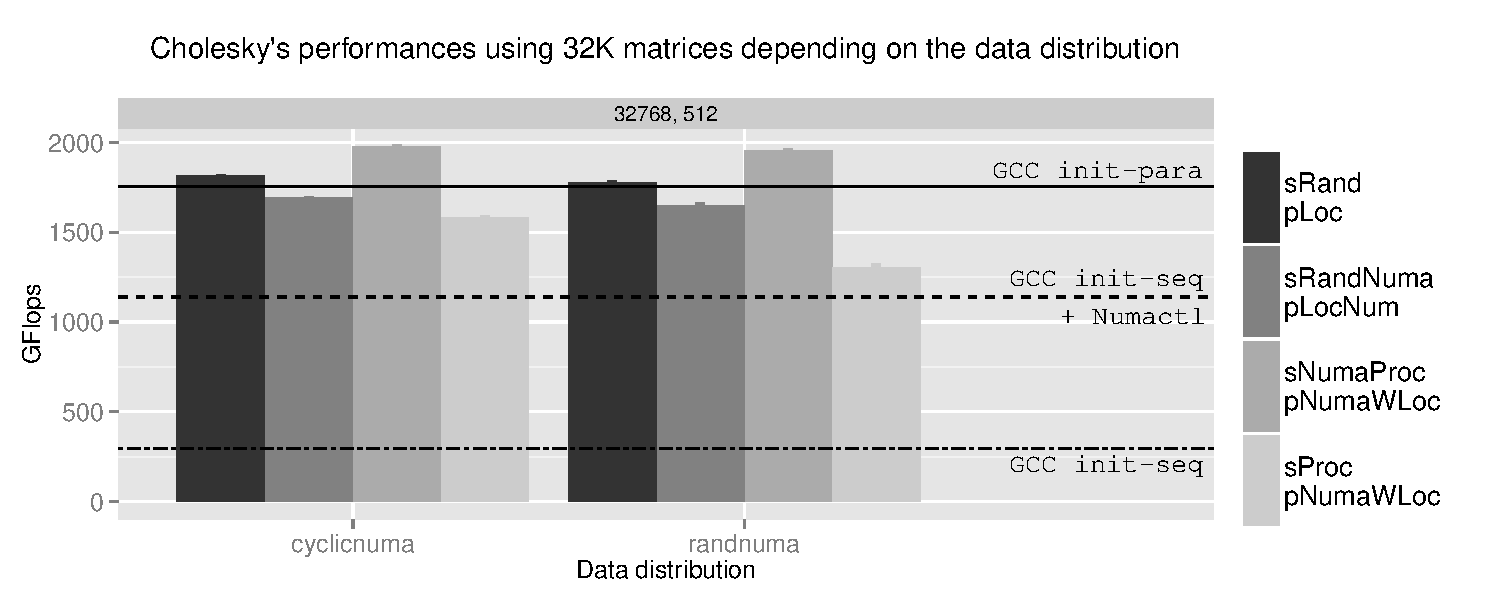
\includegraphics[scale=0.5]{figures/graph_distrib.pdf}
  \caption{Évaluation de la distribution de données pour plusieurs stratégies (WSselect + WSpush)}
\label{fig:eval-distrib}
\end{figure}

L'utilisation de \verb/numactl/ permet une amélioration significative des performances
par rapport à l'initialisation séquentielle.
En revanche l'initialisation parallèle, qu'elle soit contrôlée (\verb/cyclicnuma/,
\verb/randnuma/), ou non (GCC init-para), est nécessaire pour améliorer de
manière importante les performances.

La distribution \verb/cyclicnuma/ sera utilisée comme stratégie par défaut pour
les expériences suivantes, étant donné qu'elle offre les meilleures performances.


\subsection{Aperçu des performances des différentes stratégies}

Nous avons choisi une distribution de données, \verb/cyclicnuma/, et comparé les
différentes stratégies.
Une nouvelle fois, même si les performances obtenues ne sont évidemment pas les
même, la comparaison des stratégies les unes par rapport aux autres est similaire
pour les différentes applications que nous avons lancé.

La Figure \ref{fig:eval-all-strat} montre les résultats des expériences pour
la factorisation de Cholesky sur des matrices de largeur 32K, divisées par
bloc de 512$\times$512 éléments (meilleure taille de bloc pour cette taille de matrice).
La ligne en pointillé représente la performance du runtime de GCC,
libGOMP~\footnote{GCC 5.2.0}, en utilisant une initialisation parallèle.

La première chose à noter est que même une combinaison de stratégies \verb/WSselect/
\verb/WSpush/ basique telle que \verb/sRand/+\verb/pLoc/ obtient des performances
acceptables grâce à la distribution de données.
De plus, étant donnée une stratégie de sélection (e.g. \verb/sRandNuma/), pousser
les tâches sur le nœud NUMA où elle écrit des données (\verb/pNumaW/, \verb/pNumaWLoc/) offre
de meilleures performances que simplement pousser les tâches sur son nœud NUMA (\verb/pLocNuma/).

En considérant que les tâches sont poussées en utilisant la stratégie \verb/pNumaWLoc/,
ne prendre en compte qu'un niveau de hiérarchie (\verb/sProc/ ou \verb/sNuma/) ne permet
pas d'atteindre les performances obtenues avec des stratégies naïves. En revanche,
prendre en compte les deux niveaux de hiérarchie (\verb/sProcNuma/, \verb/sNumaProc/)
permet d'obtenir de meilleures performances que les stratégies étudiées précédemment.

\begin{figure}[t]
  \centering
  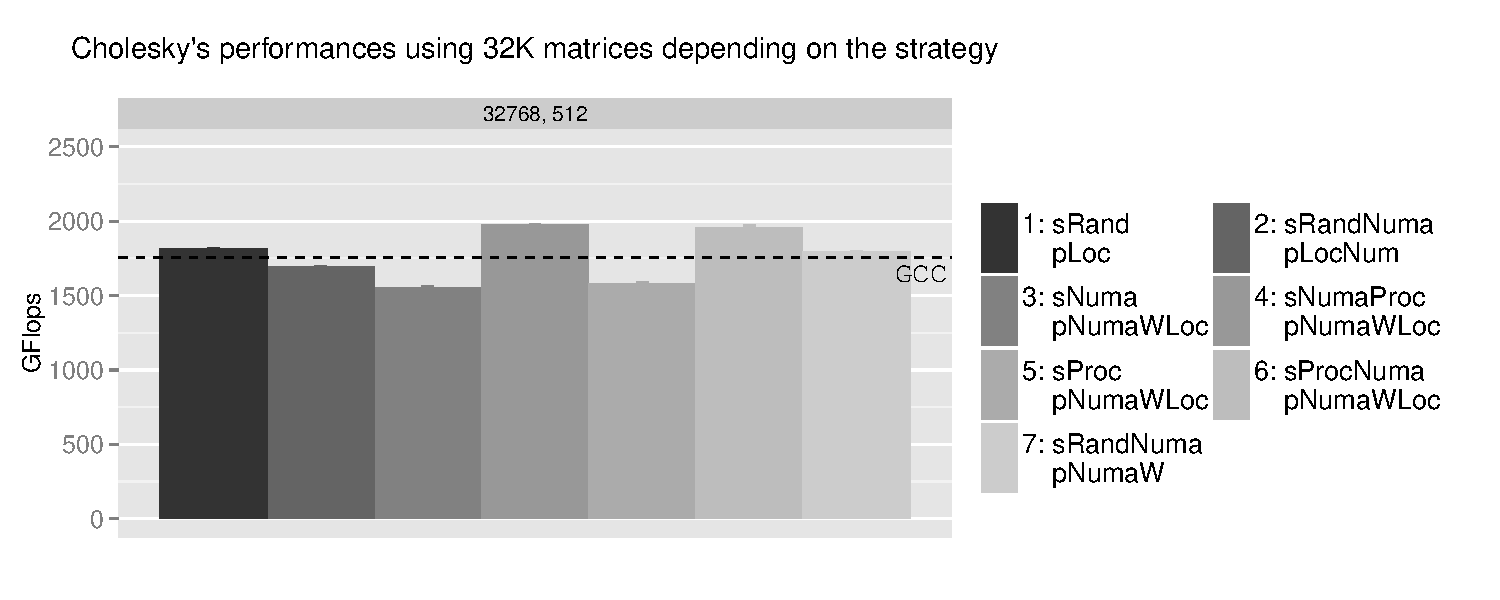
\includegraphics[scale=0.5]{figures/graph_all_strat.pdf}
  \caption{Évaluation des toutes les stratégies (WSselect + WSpush)}
\label{fig:eval-all-strat}
\end{figure}

\subsection{Scalabilité des performances des stratégies}

\begin{figure}[t]
  \centering
  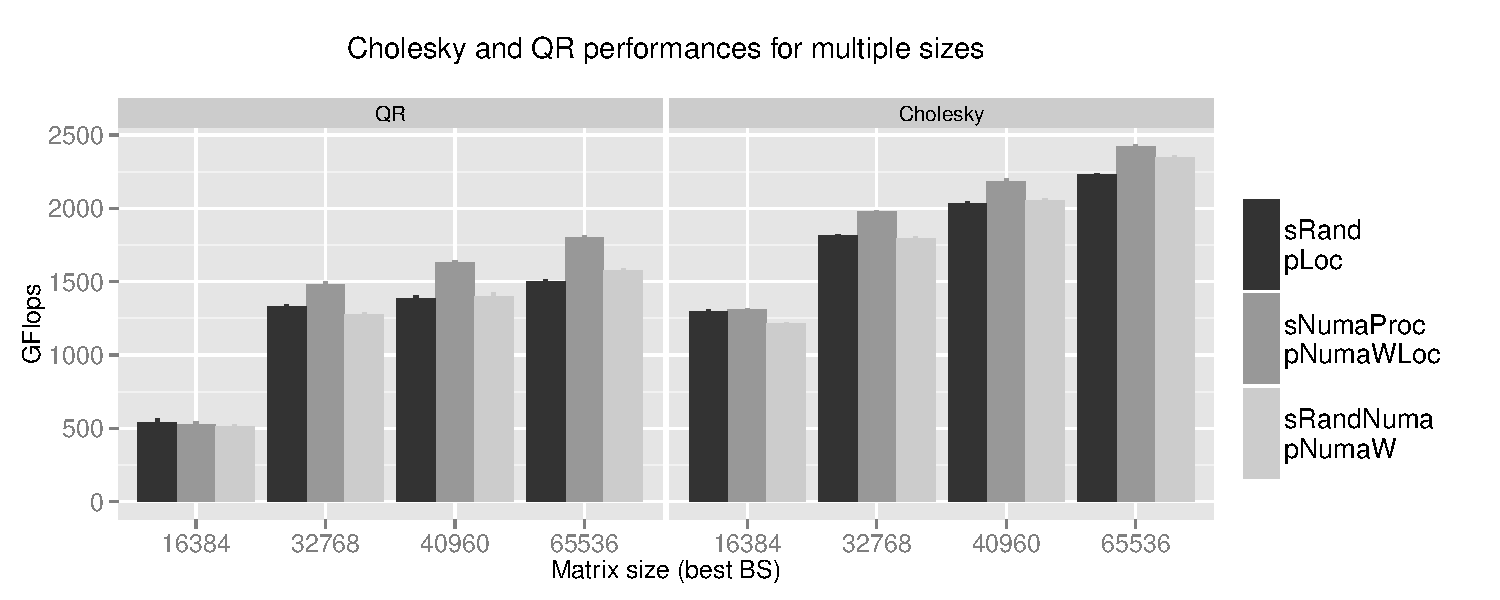
\includegraphics[scale=0.5]{figures/graph_details_strat.pdf}
\caption{Évaluation d'une sélection de stratégies sur plusieurs tailles}
\label{fig:eval-strat-sizes}
\end{figure}

Nous avons finalement sélectionné les trois combinaisons de stratégies meilleures
que les performances de GCC pour évaluer leur scalabilité en fonction de la taille
de la matrice en entrée. Ces trois combinaisons sont les suivantes :
\begin{itemize}
  \item \verb/sRand/ + \verb/pLoc/, une combinaison basique qui ne prend pas en compte la topologie.
  \item \verb/sNumaProc/ + \verb/pNumaWLoc/, la meilleure combinaison dans notre
    précédente évaluation.
  \item \verb/sRandNuma/ + \verb/pNumaW/ qui sélectionne aléatoirement
    des places au niveau NUMA.
\end{itemize}

La Figure \ref{fig:eval-strat-sizes} montre leurs performances en utilisant une distribution
\verb/cyclicnuma/.
Les performances ont été obtenues en utilisant la meilleure taille de bloc pour
chacune des tailles de matrice (qui est dans notre cas 256 pour une taille de 16384,
et 512 pour les autres).

Comme attendu, utiliser une combinaison de stratégies qui prend en compte à la fois
la localité des données et la hiérarchie de l'architecture (\verb/sNumaProc/ + \verb/pNumaWLoc/)
permet d'obtenir les meilleures performances.
La seule exception apparait pour les petites tailles de matrices (16384), où il
n'y a peut être tout simplement pas assez de travail pour tirer partie de ces stratégies. 

On peut également noter que la simple utilisation d'une distribution des données
utilisées par les tâches permet d'obtenir des performances convenables avec une
combinaison de stratégies basique (\verb/sRand/ + \verb/pLoc/).

\section{État de l'art}
\label{sec:related-work}

De nombreux travaux traitent de la localité et/ou de stratégie d'ordonnancement
spécifiques aux architectures NUMA.

Clet-Ortega et al.~\cite{DBLP:conf/europar/Clet-OrtegaCP14} ont étudié et évalué plusieurs
façon de décorer la topologie de l'architecture, en privilégiant des listes de tâches
privées par thread, parcourue de manière hiérarchique. Nos étendons ces travaux
en considérant également des listes au niveau des nœuds, et nous avons montré
que cela peut aider à améliorer les performances sur des architectures NUMA.

Olivier et al.~\cite{DBLP:journals/ijhpca/OlivierPWSP12} ont évalué des stratégies
hiérarchiques d'ordonnancement de tâches, en utilisant des structures centralisées
ou distribuées. Notamment en créant un ensemble de threads, appelé \emph{shepherd}, par
nœud NUMA, permettant à l'ordonnanceur hiérarchique d'avoir de meilleures performances
qu'avec les autres approches.

Tahan et al.~\cite{DBLP:journals/corr/Tahan14} ont également étudié le comportement
des programmes à base de tâches OpenMP sur les systèmes NUMA, en étendant le
support exécutif NANOS avec deux ordonnanceurs de tâches appellés DFWSPT et DFWSRPT,
prenant en compte la notion de priorité de tâches, et essayant également de diminuer
la distance de la mémoire lors de l'équilibrage de charge.
D'autres travaux ont été fait dans le même context~\cite{DBLP:conf/europar/TerbovenSCM12,DBLP:journals/corr/abs-1101-0093},
mais aucun ne tire partie de la clause OpenMP |depend|, qui indique précisément les
données lues et écrites par une tâches donnée. Comme montrée par notre combinaison
de stratégies \verb/sNumaProc+pNumaWLoc/, il est rentable de prendre en compte
cette information lors de l'ordonnancement.



\section{Conclusion and future work}

Les environnements de programmation à base de tâches tels qu'OpenMP sont devenus
un moyen standard de programmer des systèmes NUMA à large échelle.
Ils offrent au programmeur un moyen d'exprimer du parallélisme à grain fin,
qui peut être associé dynamiquement à la topologie de l'architecture.
OpenMP a récemment évoluer pour permettre d'exprimer les dépendances de données
entre tâches.

Ce papier présente plusieurs stratégie d'exécution pour affecter efficacement
les tâches prêtes aux listes de tâches représentant l'architecture NUMA.
Ces stratégies contrôlent à la fois la manière dont les tâches prêtes sont
initialement réparties, ainsi que la manière dont les tâches sont volées.
Nous avons évalué plusieurs distributions de données, et évalué différentes
combinaisons de stratégies "push" et "select" sur un système NUMA de 192 cœurs,
en utilisant des applications d'algèbre linéaire.
Les meilleures performances sont obtenues avec les stratégies prenant en compte à
la fois le placement initial des données et la hiérarchie de la machine.

À court terme nous prévoyons d'étendre le compilateur pour indiquer de manière
compatible avec OpenMP quelles sont les tâches d'initialisation.

Sur le long terme nous prévoyons de nous concentrer sur certaines techniques
de compilation qui pourrait nous permettre d'évaluer des informations
importantes sur les tâches, comme leur intensité opérationnelle, qui pourrait
aider à la prise de décision au sein du support exécutif. Nous pensons
que la coopération entre le compilateur et le support exécutif peut améliorer
significativement les performances et la scalabité des applications à base de tâches.

\vspace*{-2ex}
\section*{Acknowledgments}

PIA ELCI - Projet financé par le gouvernement français pour le développement
des applications hautes performances.

\bibliography{Bib/paper.bib}

\end{document}






